\subsection{Defining Extreme, Critical, and Saddle Points}
Let $f: U \subseteq \R^n \rightarrow \R^m$, where $U$ is an open set.

\begin{defn}[Local Maxima and Minima]
    We say that,
    \begin{enumerate}
        \sloppy
        \item $f$ has a \textbf{local maximum} at $\mathbf{x}_0$ if there exists an open neighborhood $N$ of $\mathbf{x}_0$ such that $f(x) \geq f(\mathbf{x}_0)$ for all $x \in N$
        \item $f$ has a \textbf{local minimum} at $\mathbf{x}_0$ if there exists an open neighborhood $N$ of $\mathbf{x}_0$ such that $f(x) \leq f(\mathbf{x}_0)$  for all $x \in N$
    \end{enumerate}
    The local extremum are called \textbf{strict} if the inequalities are strict.
\end{defn}

\begin{marginfigure}
    Extrema can be \textbf{local} or \textbf{global}. Depending on the choice of $U$, these extrema may or may not be captured by the first-derivative test.
\end{marginfigure}

\begin{defn}[Critical Points]
    There are (3) types of critical points,
    \begin{itemize}
        \item $\mathbf{x}_0 \in U$ is \textbf{extreme} if $\mathbf{x}_0$ is a local minimum or maximum
        \item $\mathbf{x}_0 \in U$ is \textbf{critical} if,
        \begin{itemize}
            \item $f$ is not differentiable at $\mathbf{x}_0$
            \item $f$ is differentiable at $\mathbf{x}_0$ and
            \[(\mathbf{D} f)(\mathbf{x}_0) = 0 \iff \left(\mathbf{\nabla}_{\mathbf{v}} f\right)\left(\mathbf{x}_0\right) = 0\]
        \end{itemize}
        \item $\mathbf{x}_0 \in U$ is a \textbf{saddle point} if $\mathbf{x}_0$ is critical but not extreme
    \end{itemize}
\end{defn}

\subsection{First-Derivative Test for Local Extrema}
\begin{thm}[First-Derivative Test for Local Extrema]
   Let $\mathbf{x}_0$ be a local maximum or minimum. If $f$ is differentiable at $\mathbf{x}_0$, then $\mathbf{D} f\left(\mathrm{x}_0\right)=0$.
\end{thm}

\begin{proof}
   Suppose that $f$ achieves a local maximum at $\mathbf{x}_0$.
   \begin{enumerate}
       \item If $m = 1$, then for any $\mathbf{h} \in \R^n$, the function $g(t) = f(\mathbf{x}_0, t\mathbf{h})$ has a local maximum at $t = 0$. From one-variable calculus,
       \[g^{\prime}(0) = 0\]
       By the chain rule,
       \[g^{\prime}(0)=\left[(\mathbf{D} f)\left(\mathbf{x}_0\right)\right] \cdot \mathbf{h} = 0\]
       This implies that $\operatorname{D} f\left(\mathbf{x}_0\right)=\mathbf{0}$.
        \item If $m > 1$, then we can use the same idea. Given $\mathbf{x}_0$ and $\mathbf{h}$ fixed,
        \[\frac{d}{d t} f\left(\mathbf{x_0}+t \mathbf{h}\right)=(\mathbf{\nabla} f)\left(\mathbf{x_0}+t \mathbf{h}\right) \cdot \mathbf{h}\]
        Evaluated at $t = 0$,
        \[0=(\mathbf{\nabla f})\left(\mathbf{x_0}\right) \cdot \mathbf{h} \Rightarrow(\mathbf{\nabla f})\left(\mathbf{x_0}\right)=0\]
         \begin{center}
            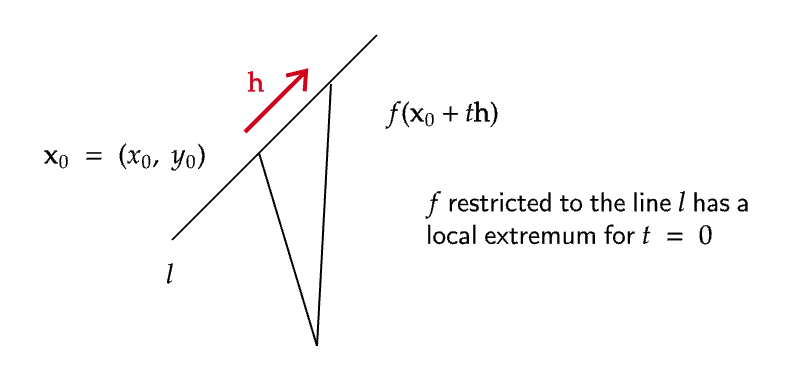
\includegraphics[width=0.9\linewidth]{figures/wk-3/fig-36.png}
        \end{center}
   \end{enumerate}
   The case where $f$ achieves a local minimum is analogous.
\end{proof}

\begin{ex}{Critical Points which are not Local Extremum}{label}
    The function $f: \R^2 \rightarrow \R$ defined by 
    \[f(x,y) = xy\]
    has $(0,0)$ as a critical point, but it is not a local extremum.
\end{ex}

\begin{marginfigure}
    Functions can have many critical points:
    \begin{center}
        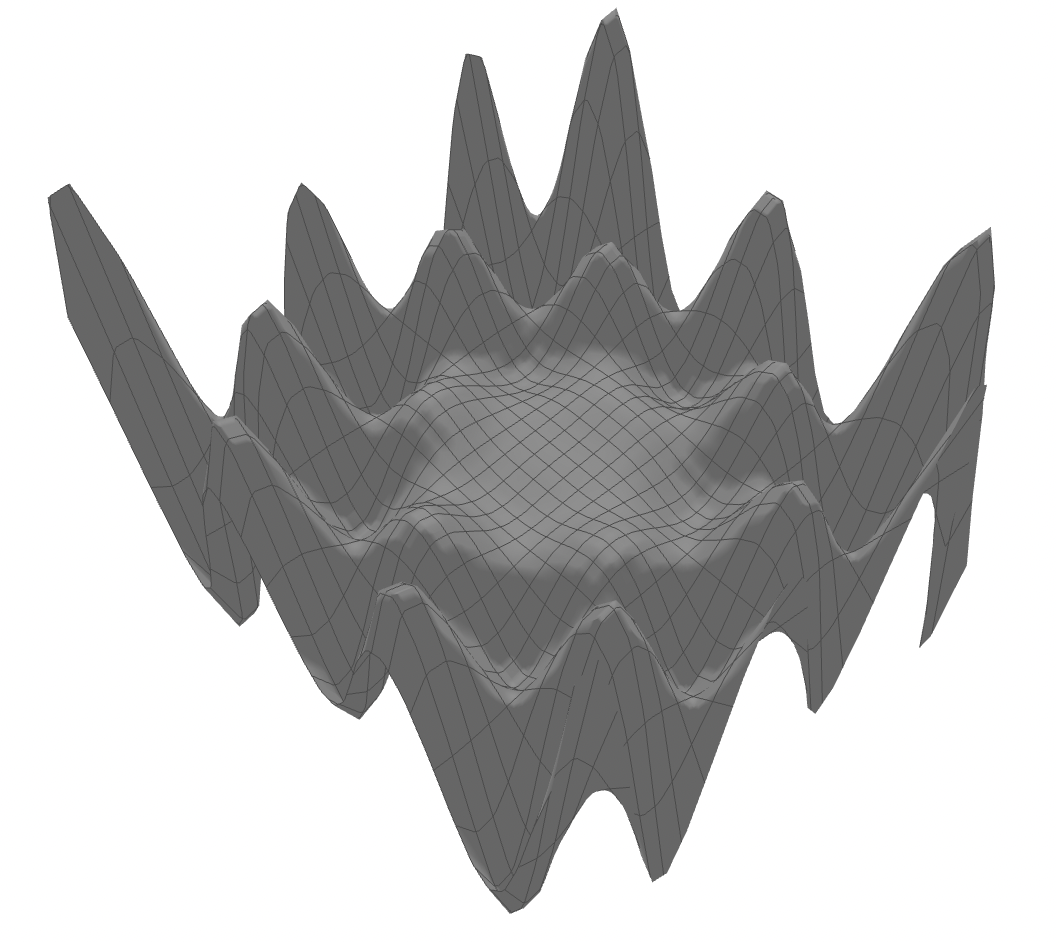
\includegraphics[width=0.7\linewidth]{figures/wk-3/fig-35.png}
    \end{center}
\end{marginfigure}

\begin{ex}{Geometric Interpretation of Critical Points}{label}
    \begin{center}
        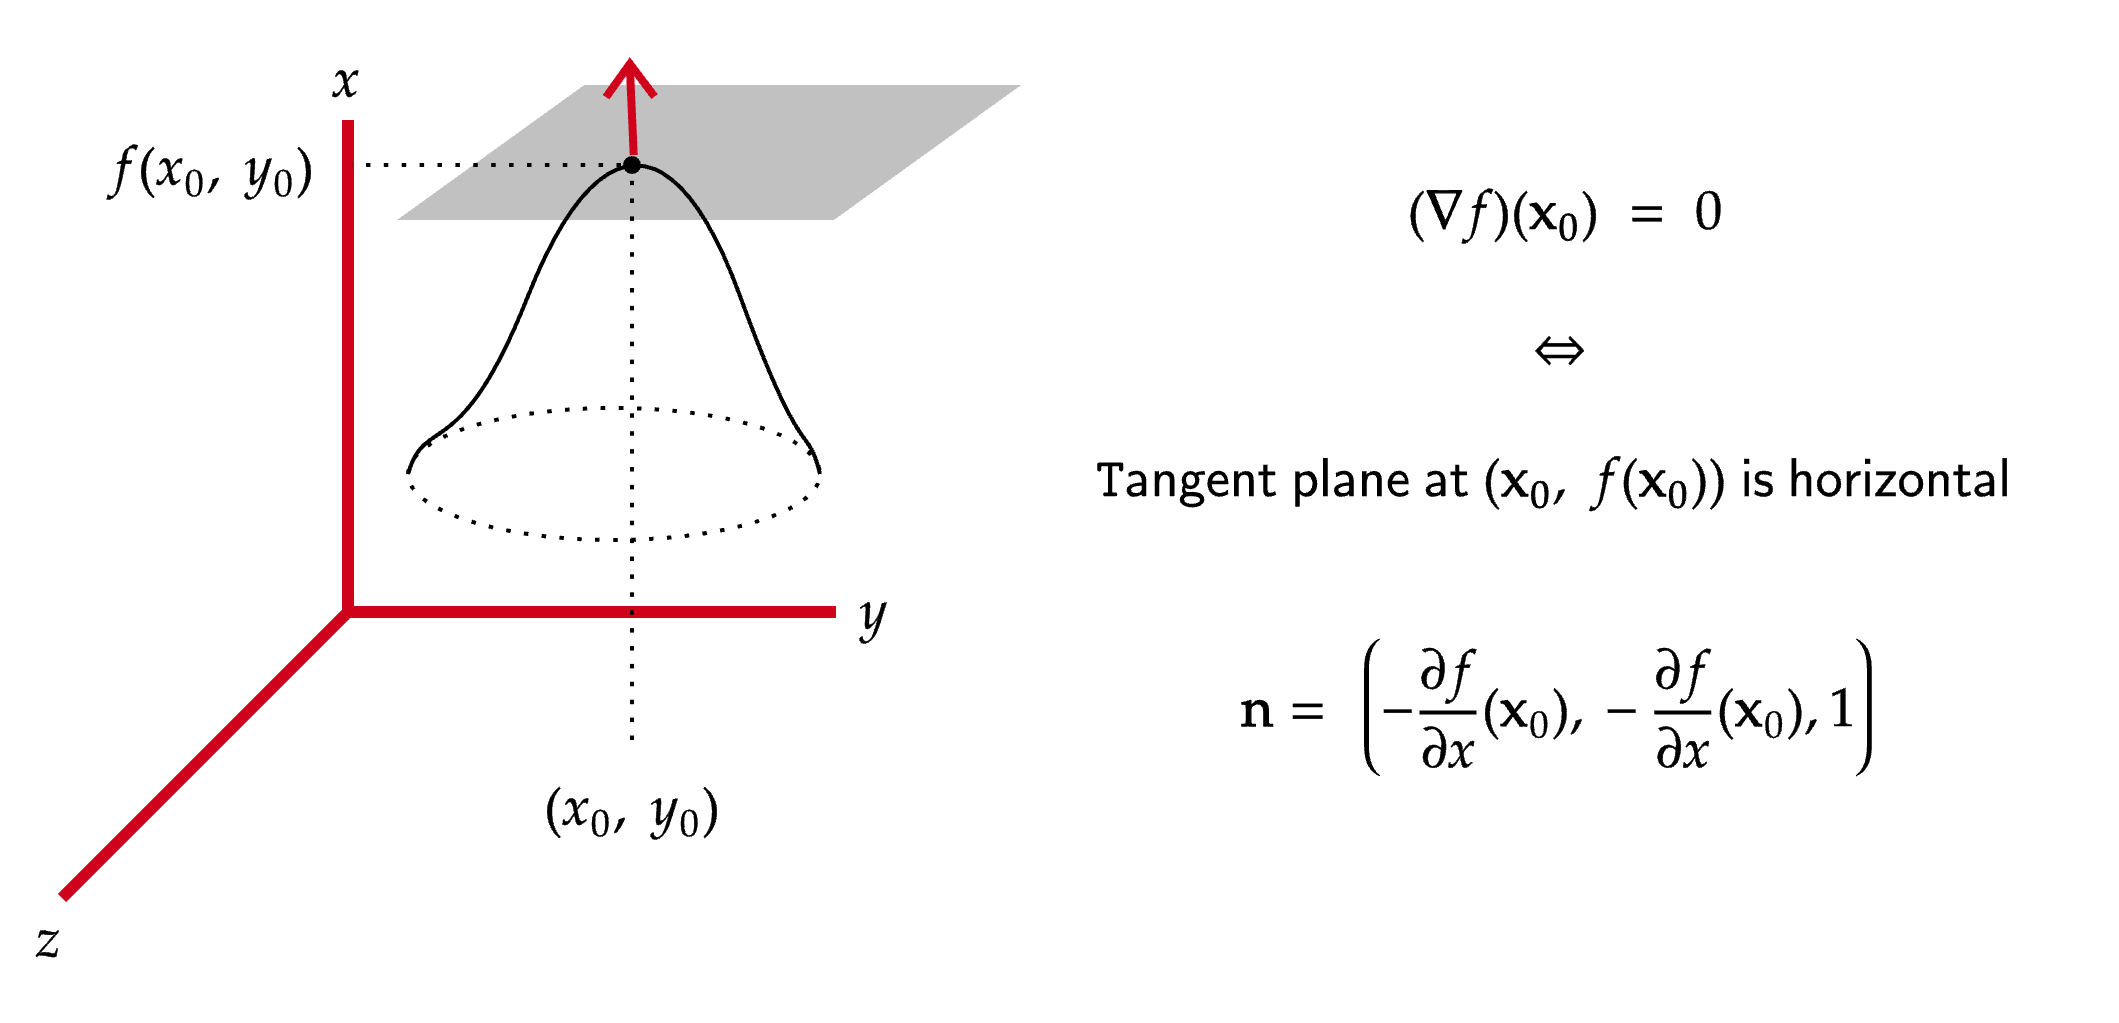
\includegraphics[width=\linewidth]{figures/wk-3/fig-37.png}
    \end{center}
\end{ex}

\subsection{Second Derivative Test}
We will establish an analog of the \textbf{second derivative test}. At a critical point $\mathbf{x}_0$, Taylor's Theorem tells us that,
\[f\left(\mathbf{x}_0+\mathbf{h}\right)=f\left(\mathbf{x}_0\right)+\sum_{i=1}^n \frac{\partial f}{\partial x_i}\left(\mathbf{x_0}\right) h_i+ \frac{1}{2} \cdot \sum_{i, j=1}^n \frac{\partial^2 f}{\partial x_i x_j}\left(\mathbf{x_0}\right) h_i h_j+R_2\left(\mathbf{x}_0, \mathbf{h}\right)\]
implying in particular that,
\[f\left(\mathbf{x}_0+\mathbf{h}\right)-f\left(\mathbf{x}_0\right)= \frac{1}{2} \sum_{i, j} \underbrace{\frac{\partial^2 f}{\partial x_i x_j}\left(\mathbf{x_0}\right) h_i h_j}_{(*)}+R_2\left(\mathbf{x_0}, \mathbf{h}\right)\]
where $(*)$ is quadratic in $\mathbf{h}$ and the remainder decays faster than quadratically. We require the following \textbf{algebraic terminology}:

\begin{defn}[Quadratic Function]
    A function $g: \R^n \rightarrow \R$ defined
    \[g\left(h_1, \ldots, h_n\right) = \sum_{i, j=1}^n a_{i j} h_i h_j\]
    for an $n \times n$ matrix $\mathbf{A}$ with entries $a_{i j}$ is called \textbf{quadratic}.
\end{defn}

\begin{ex}{Quadratic Function: $n = 3$}{label}
    \begin{align*}
        g\left(h_1, h_2, h_3\right)
        &=\left[h_1, h_2, h_3\right]\left[\begin{array}{rrr}
        1 & -1 & 0 \\
        -1 & 0 & 0 \\
        0 & 0 & 1
        \end{array}\right]\left[\begin{array}{l}
        h_1 \\
        h_2 \\
        h_3
        \end{array}\right] \\
        &=h_1^2-2 h_1 h_2+h_3^2
        \end{align*}
\end{ex}

\begin{prop}[Properties of Quadratic Forms]
    Observe that,
    \begin{enumerate}
        \item $g$ is homogeneous of degree 2,
        \[g(\lambda h_1, \cdots \lambda h_n) = \lambda^2 g(h_1, \cdots, h_n)\]
        \item We may assume that the matrix $\mathbf{A}$ is symmetric, i.e., $a_{ij} = a{ji}$ for all $i, j$. If not, then we can write
        \[a_{ij} = \frac{1}{2}\underbrace{(a_{ij} + a_{ji})}_{b_{ij}} + \frac{1}{2}\underbrace{(a_{ij} - a_{ji})}_{c_{ij}}\]
        where $b_{ij} = b_{ji}$ (symmetric) and $c_{ij} = -c_{ji}$ (skew-symmetric).
        \[\sum a_{i j} \cdot h_i h_j=\sum b_{i j} \cdot h_i h_j+\overbrace{\sum c_{i j} \cdot h_i h_j}^{=0}\]
        and choose the symmetric matrix $\mathbf{B}$.
    \end{enumerate}
\end{prop}

\begin{marginfigure}
    Every matrix can be written as a function of a symmetric matrix and a skew symmetric matrix.
\end{marginfigure}

\begin{defn}[Positive and Negative Definite]
     A quadratic form is
     \begin{itemize}
         \item \textbf{Positive definite} if $g(\mathbf{h}) \geq 0$ for all $\mathbf{h} \in \R^n$
         \item \textbf{Negative definite} if $g(\mathbf{h}) \leq 0$ for all $\mathbf{h} \in \R^n$
     \end{itemize}
     with the added condition that $g(\mathbf{h}) = 0$ if and only if $\mathbf{h} = 0$.
\end{defn}

\begin{defn}[Hessian]
    Suppose that $f: U \subseteq \R^n \rightarrow \R$ has second-order continuous derivatives at $\mathbf{x}_0 \in U$. The \textbf{Hessian} of $f$ at $\mathbf{x}_0$ is
    \begin{align*}
        (\mathbf{H} f) \left(\mathrm{x}_0\right)(\mathbf{h}) &= \frac{1}{2} \cdot \sum_{i, j=1}^n \frac{\partial^2 f}{\partial x_i \partial x_j}\left(\mathbf{x}_0\right) h_i h_j \\
        &=\frac{1}{2}\left[h_1, \ldots, h_n\right]\left[\begin{array}{ccc}
        \frac{\partial^2 f}{\partial x_1 \partial x_1} & \cdots & \frac{\partial^2 f}{\partial x_1 \partial x_n} \\
        \vdots & & \\
        \frac{\partial^2 f}{\partial x_n \partial x_1} & \cdots & \frac{\partial^2 f}{\partial x_n \partial x_n}
        \end{array}\right]\left[\begin{array}{c}
        h_1 \\
        \vdots \\
        h_n
        \end{array}\right]
    \end{align*}
    which is a quadratic function by equality of the mixed partials. 
\end{defn}

\begin{table}[h]
\begin{tabularx}{\textwidth}{ccc}
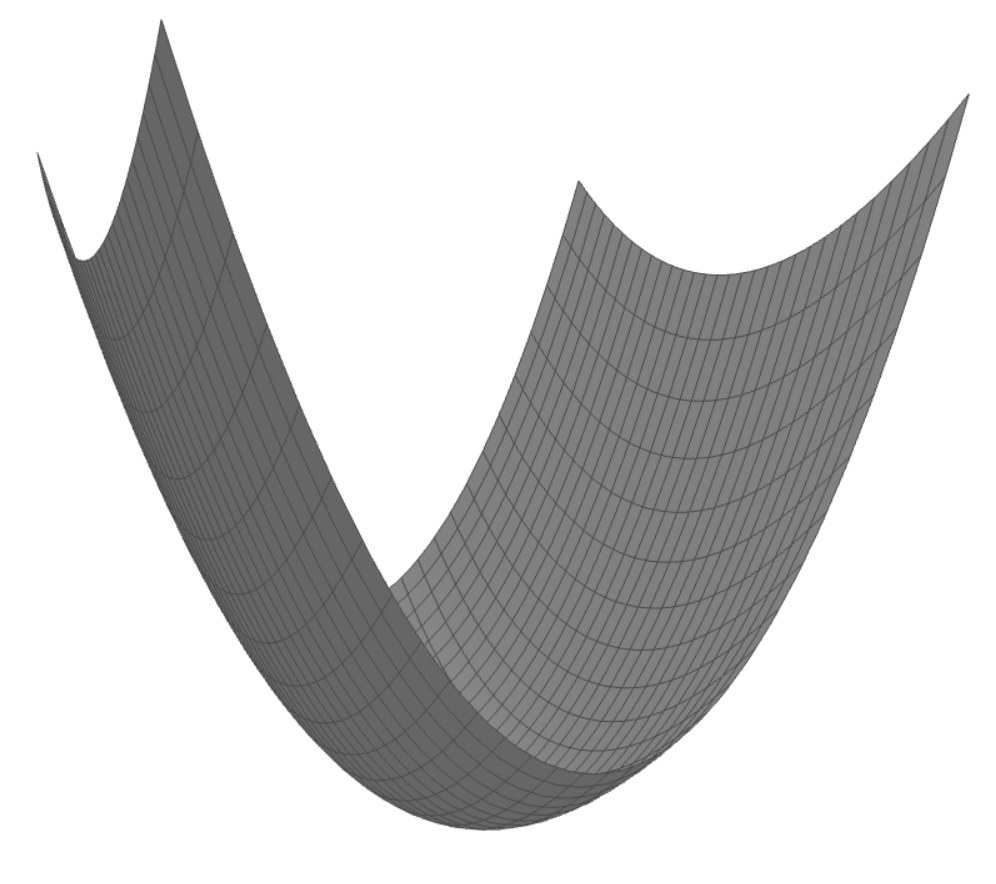
\includegraphics[width=0.3\linewidth]{figures/wk-3/fig-39.png} & 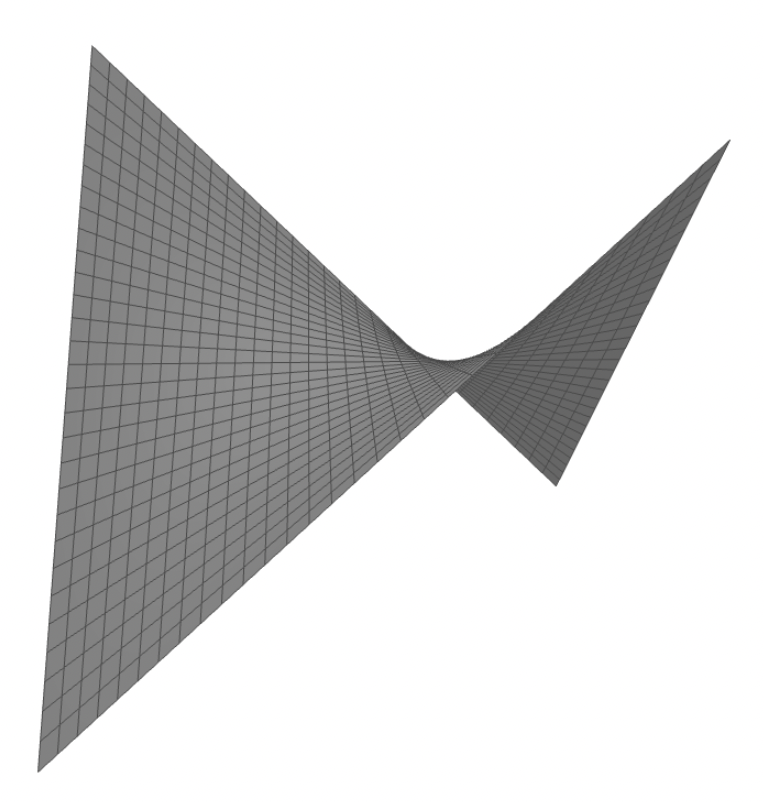
\includegraphics[width=0.3\linewidth]{figures/wk-3/fig-40.png} & 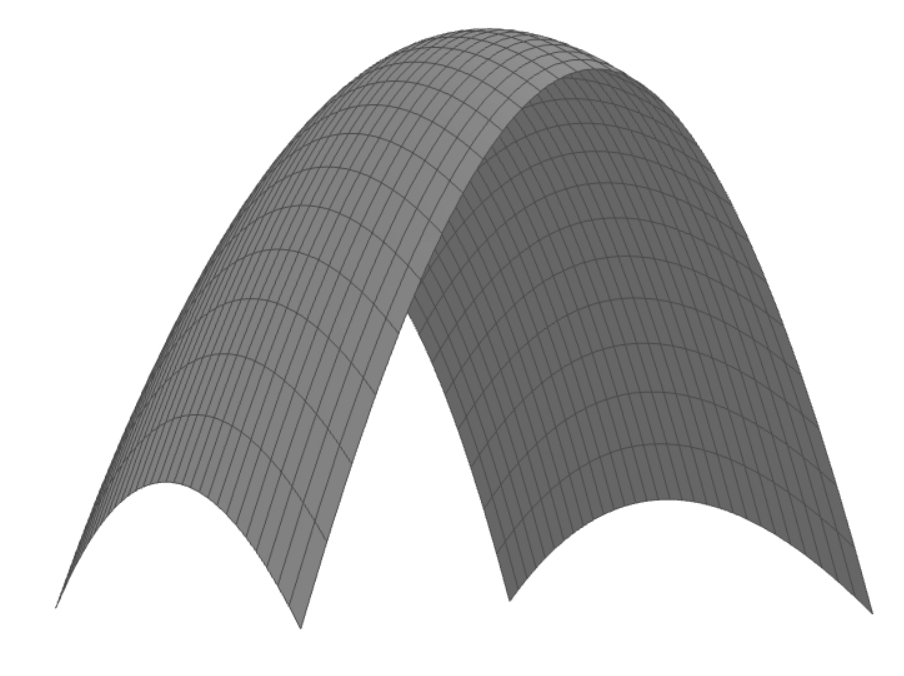
\includegraphics[width=0.3\linewidth]{figures/wk-3/fig-41.png} \\ \\
$g(\mathbf{h})=h_1^2+h_2^2$ & $g(\mathbf{h})=h_1^2 \cdot h_2^2$ & $g(\mathbf{h})=-h_1^2-h_2^2$ \\ \\
$\boldsymbol{A}=\left(\begin{array}{ll}1 & 0 \\ 0 & 1\end{array}\right)$ & $\boldsymbol{A}=\left(\begin{array}{ll}0 & \frac{1}{2} \\ \frac{1}{2} & 0\end{array}\right)$ & $\boldsymbol{A}=\left(\begin{array}{cc}-1 & 0 \\ 0 & -1\end{array}\right)$ \\ \\
Positive Definite & Neither & Negative Definite
\end{tabularx}
\end{table}

\begin{prop}
    Let $g: \R^n \rightarrow \R$ be a positive definite quadratic form. There exists a constant $M > 0$ such that,
    \[g(\mathbf{h}) \geq M \cdot \|\mathbf{h}\|^2\]
\end{prop}

\begin{thm}[Second Derivative Test]
   Let $f: U \subseteq \R^n \rightarrow \R$ be a function of class $C^3$. Consider a critical point $\mathbf{x}_0$ of $f$. Then,
   \[
   (\mathbf{H}(f))\left(\mathbf{x}_0\right)(\mathbf{h})=\left\{\begin{array}{l}\text { Positive Definite } \Rightarrow \mathbf{x}_0 \text { is a local minimum } \\ \text { Negative Definite } \Rightarrow \mathbf{x}_0 \text { is a local maximum }\end{array}\right.
   \]
\end{thm}

\begin{proof}
    If $f: U \subseteq \R^n \rightarrow \R$ is of class $C^3$, then,
    \[f(\mathbf{x}_0 + \mathbf{h}) - f(\mathbf{x}_0) = (\mathbf{H}f)(\mathbf{x}_0)(\mathbf{h}) + R_2(\mathbf{x}_0, \mathbf{h})\]
    by Taylor's Theorem, where $R_2(\mathbf{x}_0, \mathbf{h} / \|\mathbf{h}\|^2 \rightarrow \mathbf{0}$ as $\mathbf{h} \rightarrow \mathbf{0}$ and $\mathbf{x}_0 \in U$ is a critical point. Since $(\mathbf{H}f)(\mathbf{x}_0)(\mathbf{h})$ is positive definite,
    \[(\mathbf{H}f)(\mathbf{x}_0)(\mathbf{h}) \geq M \cdot \|\mathbf{h}\|^2\]
    for some $M > 0$. There exists $\delta > 0$ such that for $0 < \|\mathbf{h}\| < \delta$, 
    \[|R_2(\mathbf{x}_0, \mathbf{h}| < M \cdot \|\mathbf{h}\|^2\]
    Thus, $0< (\mathbf{H}f) \left(\mathbf{x}_0\right)(\mathbf{h})+R_2\left(\mathbf{x}_0, \mathbf{h}\right)=f\left(\mathbf{x}_0+\mathbf{h}\right)-f\left(\mathbf{x}_0\right)$ for $0<\|\mathbf{h}\|<\delta$. It follows that $\mathbf{x}_0$ is a strict relative minimum. The negative definite case follows by applying this argument to $-f$.
\end{proof}

\begin{marginfigure}
\begin{center}
    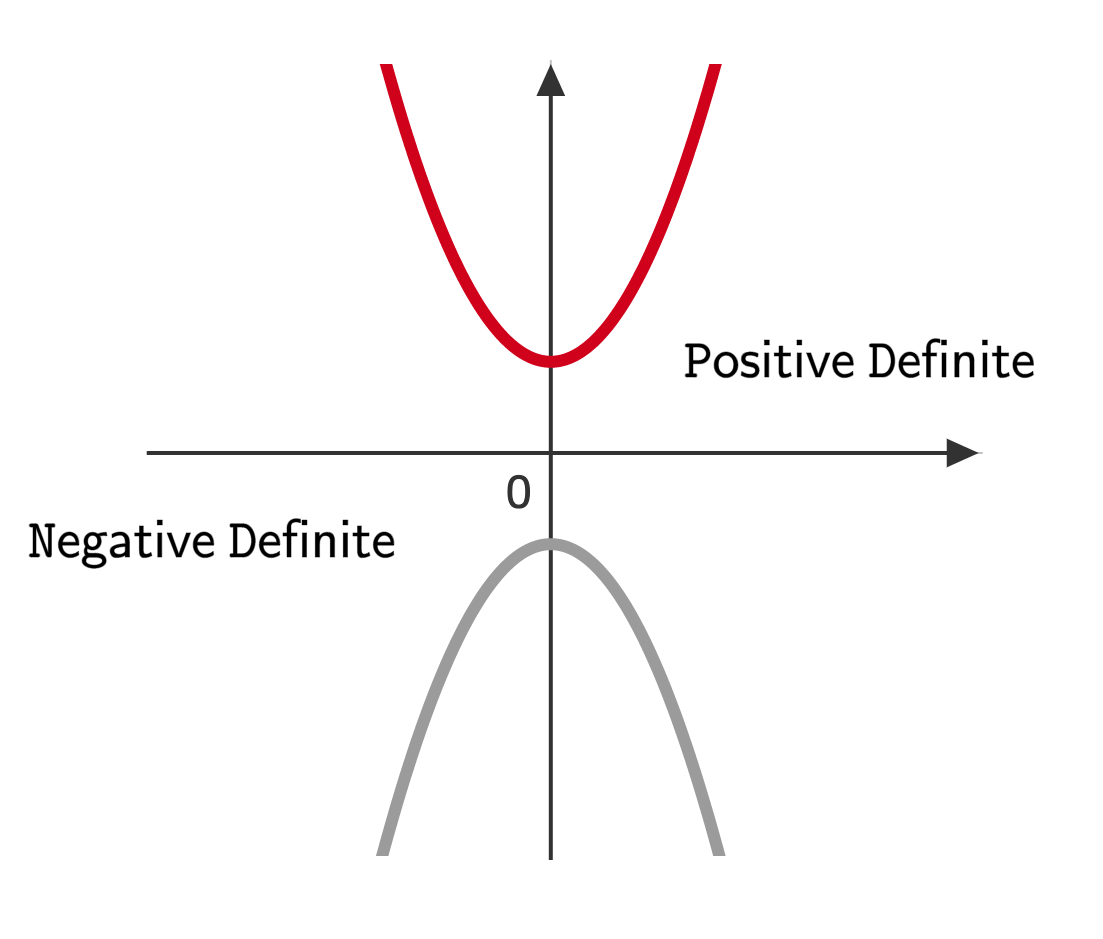
\includegraphics[width=0.7\linewidth]{figures/wk-4/fig-42.png}
\end{center}
\end{marginfigure}

\begin{prop}
     For a quadratic form $g(h_1, h_2)$,
    \begin{align*}
        &a > 0 \text{ and } ac-b^2 > 0 \iff \text{Positive Definite}\\
        &a < 0 \text{ and } ac-b^2 > 0 \iff \text{Negative Definite}
    \end{align*}
\end{prop}

\begin{proof}
    Take
    \[g(h_1, h_2) = \left( \begin{array}{cc}
         h_1 & h_2
    \end{array}\right) \left(\begin{array}{cc}
        a & b \\
        c & d
    \end{array}\right)\left( \begin{array}{c}
         h_1 \\ h_2
    \end{array}\right)\]
    Expanding this expression gives that,
    \[g(h_1, h_2) = ah_1^2 + 2bh_1h_2 + ch_2^2\]
    Completing the square:
    \[g\left(h_1, h_2\right)=\frac{1}{2} a\left(h_1+\frac{b}{a} h_2\right)^2+\frac{1}{2}\left(c-\frac{b^2}{a}\right) h_2^2\]
    Suppose that $g$ is positive definite.
    \begin{align*}
    &h_2=0 \Rightarrow \frac{1}{2} a h_1^2 \Rightarrow a>0 \\
    &h_1=-\frac{b}{a} h_2 \Rightarrow \frac{1}{2} \underbrace{\left(c-\frac{b^2}{a}\right)}_{>0} h_2^2
    \end{align*}
    Conversely,
    \[a > 0 \text{ and } ac-b^2 > 0 \implies g\left(h_1, h_2\right) > 0\]
    since we sum over positive numbers.
\end{proof}


\begin{rmk}[Determinant Test]
    Let $n \geq 0$ and consider
   \[g(\mathbf{h}) = \sum_{i,j=1}^n a_{ij} h_i h_j\]
   with entries taken from the symmetric matrix
   \[\mathbf{A} = \left(\begin{array}{cccc}
    a_{11} & a_{12} & \cdots & a_{1 n} \\
    a_{21} & a_{22} & \cdots & a_{2 n} \\
    a_{31} & a_{32} & \cdots & a_{3 n} \\
    \vdots & & & a_{n n}
    \end{array}\right)\]
    With reference to the margin figure,
    \begin{enumerate}
        \item $g$ is positive definite if the determinants of every diagonal embedded minor are positive
        \item $g$ is negative definite if the determinants of every diagonal embedded minor alternate signs
    \end{enumerate}
\end{rmk}

\begin{marginfigure}
Diagonal embedded minors of $\mathbf{A}$
\begin{center}
    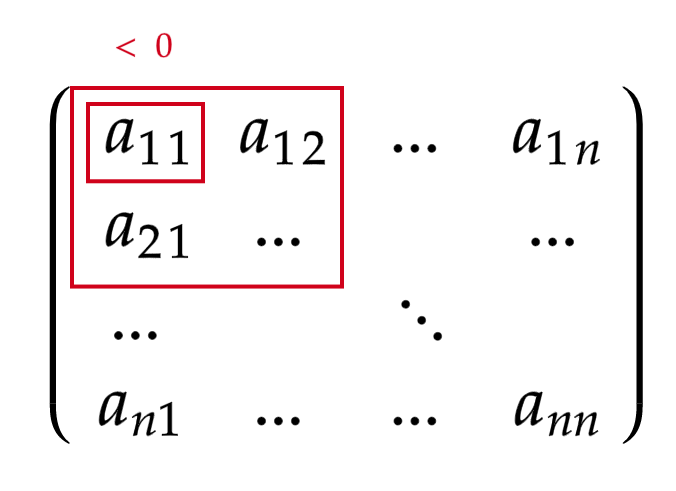
\includegraphics[width=0.7\linewidth]{figures/wk-4/fig-43.png}
\end{center}
\end{marginfigure}

\begin{thm}[Second-Derivative Test]
    Let $f: U \subseteq \R^2 \rightarrow \R$.
    \begin{itemize}
        \item $\mathbf{x}$ is a \textbf{local minimum} of $f$ if,
        \begin{enumerate}
            \item $f_x(\mathbf{x}) = f_y(\mathbf{x}) = 0$
            \item $f_{xx}(\mathbf{x}) > 0$
            \item $(f_{xx} \cdot f_{yy} - f_{xy}^2)(\mathbf{x}) > 0$
        \end{enumerate}
        \item $\mathbf{x}$ is a \textbf{local maximum} of $f$ if,
        \begin{enumerate}
            \item $f_x(\mathbf{x}) = f_y(\mathbf{x}) = 0$
            \item $f_{xx}(\mathbf{x}) < 0$
            \item $(f_{xx} \cdot f_{yy} - f_{xy}^2)(\mathbf{x}) > 0$
        \end{enumerate}
        \item $\mathbf{x}$ is a \textbf{saddle type} of $f$ if,
        \begin{enumerate}
            \item $(f_{xx} \cdot f_{yy} - f_{xy}^2)(\mathbf{x}) < 0$
        \end{enumerate}
    \end{itemize}
    with the \textbf{indeterminant} case occuring when,
    \[(f_{xx} \cdot f_{yy} - f_{xy}^2)(\mathbf{x}) = 0\]
\end{thm}

\begin{ex}{$f(x, y)=x^2-y^2+x y$}{label}
Consider the function,
\begin{align*}
&f(x, y)=x^2-y^2+x y \\
&f_x=2 x+y=0 \quad \text{ and } \quad f_y=-2 y+x=0
\end{align*}
$(0,0)$ is the unique critical point. Computing the Hessian,
\[\left|\left(\begin{array}{ll}
f_{x x} & f_{x y} \\
f_{x y} & f_{y y}
\end{array}\right)\right|=\left|\left(\begin{array}{cc}
2 & 1 \\
1 & -2
\end{array}\right)\right|=\left(f_{x x} \cdot f_{y y}-f_{x y}^2\right)(0,0)=-5\]
shows that $(0,0)$ is a saddle point.
\end{ex}

\begin{marginfigure}
$f(x,y) = x^2-y^2+x y$
\begin{center}
    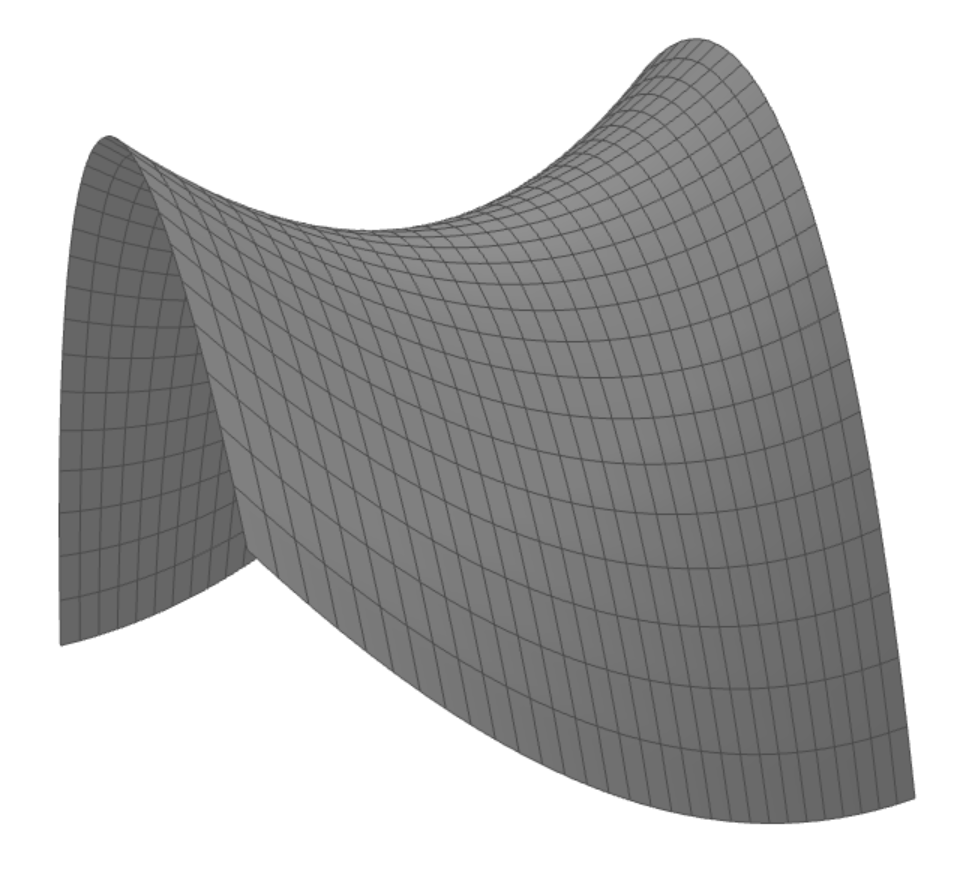
\includegraphics[width=0.7\linewidth]{figures/wk-4/fig-44.png}
\end{center}
$f(x,y) =e^x \cdot \cos y$
\begin{center}
    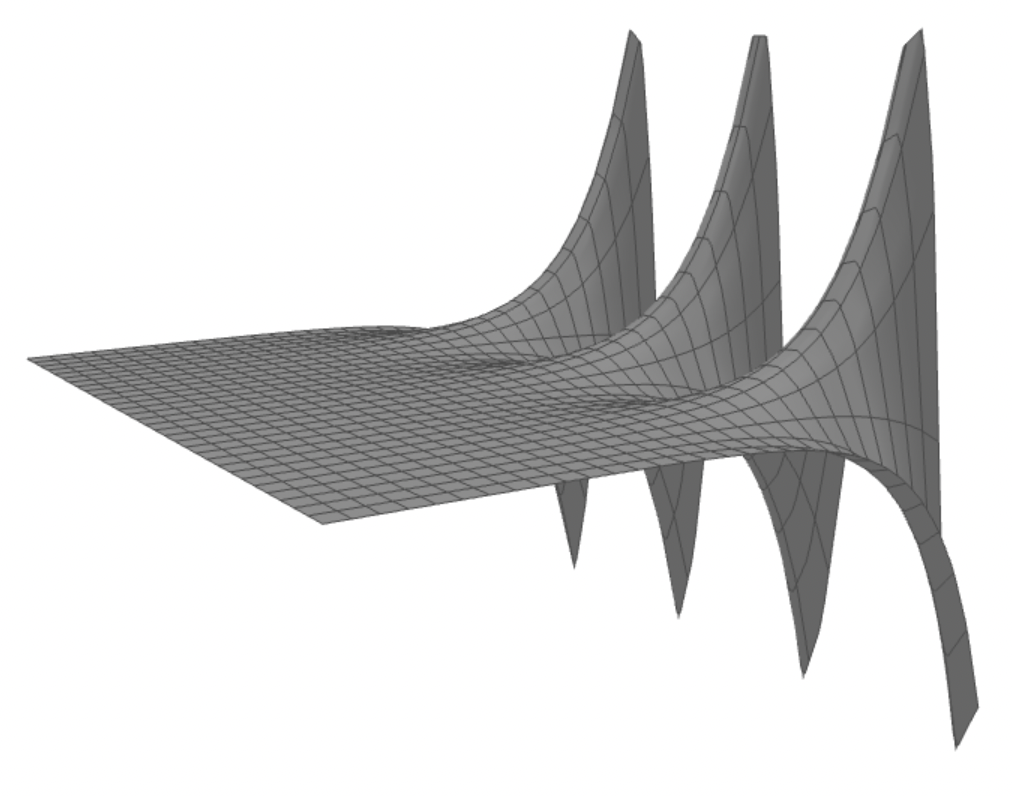
\includegraphics[width=0.7\linewidth]{figures/wk-4/fig-45.png}
\end{center}
$\frac{1}{3} x^3+\frac{1}{3} y^3-\frac{1}{2} x^2-\frac{5}{2} y^2+x y+10$
\begin{center}
    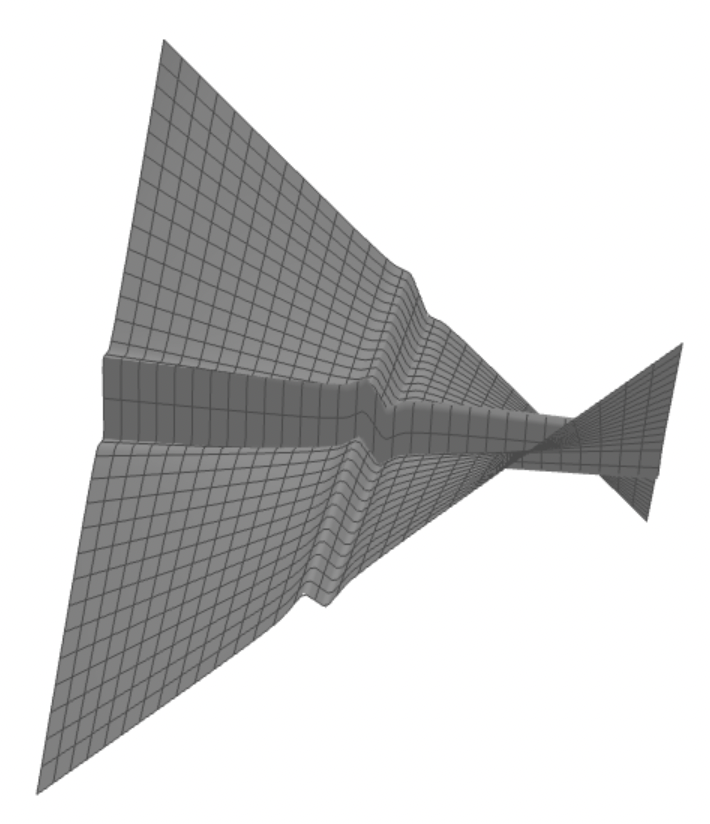
\includegraphics[width=0.7\linewidth]{figures/wk-4/fig-46.png}
\end{center}
$f(x,y) =xy+\frac{1}{x}+\frac{1}{y}$
\begin{center}
    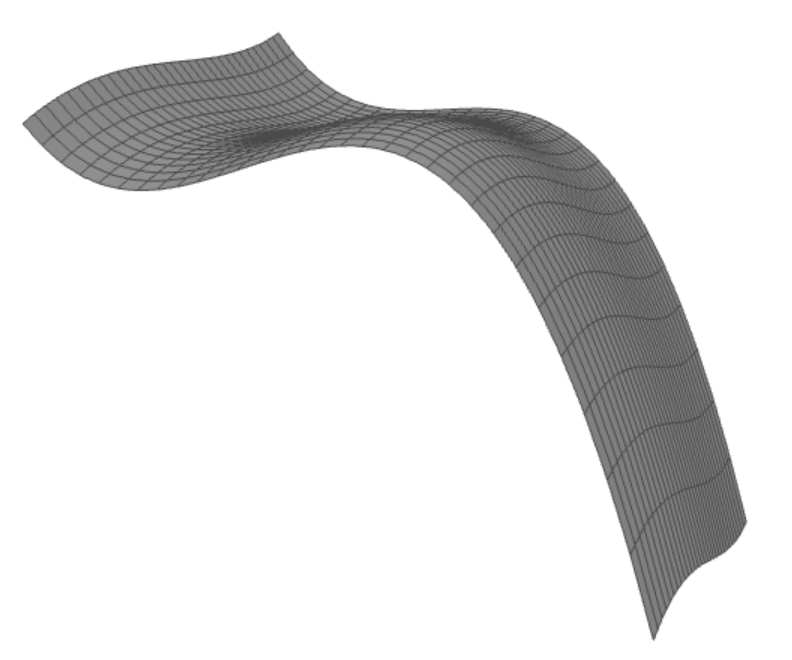
\includegraphics[width=0.7\linewidth]{figures/wk-4/fig-47.png}
\end{center}
\end{marginfigure}

\begin{ex}{$f(x, y)=e^x$}{label}
Consider the function,
\begin{align*}
&f(x, y)=e^x \cdot \cos y \\
&f_x=e^x \cos y \quad \text { and } \quad f_y=e^x \sin y
\end{align*}
$f$ has no critical points.
\end{ex}

\begin{ex}{$f(x, y)=x y+\frac{1}{x}+\frac{1}{y}$}{label}
Consider the function,
\begin{align*}
&f(x, y)=x y+\frac{1}{x}+\frac{1}{y} \\
&f_x=y-\frac{1}{x^2} \quad \text{ and } \quad f_y=x-\frac{1}{y^2}
\end{align*}
$(1,1)$ is the unique critical point. Computing the Hessian,
\[
\left|\left(\begin{array}{cc}
f_{x x} & f_{x y} \\
f_{x y} & f_{y y}
\end{array}\right)\left(x_0, y_0\right)\right|=\left|\left(\begin{array}{cc}
\frac{2}{x^3} & 1 \\
1 & \frac{2}{y^3}
\end{array}\right)(1,1)\right|=\left|\left(\begin{array}{cc}
2 & 1 \\
1 & 2
\end{array}\right)\right|=3
\]
shows that $(1,1)$ is a local minimum.
\end{ex}

\begin{ex}{$f(x, y)=\frac{1}{3} x^3+\frac{1}{3} y^3-\frac{1}{2} x^2-\frac{5}{2} y^2+x y+10$}{label}
Consider the function,
\begin{align*}
&f(x, y)=\frac{1}{3} x^3+\frac{1}{3} y^3-\frac{1}{2} x^2-\frac{5}{2} y^2+x y+10\\
&f_x=x^2-x \quad \text{ and } \quad f_y=y^2-5 y+6
\end{align*}
$(0,2)$,$(0,3)$, $(1,2)$, and $(1,3)$ are critical points.
\[\left(\begin{array}{ll}
f_{x x} & f_{x y} \\
f_{x y} & f_{y y}
\end{array}\right)=\left(\begin{array}{cc}
2 x-1 & 0 \\
0 & 2 y-5
\end{array}\right)\]
shows that,
\begin{align*}
    &(0,2) \text{ is a local minimum} \\
    &(0,3) \text{ is a saddle point} \\
    &(1,2) \text{ is a saddle point} \\
    &(1,3) \text{ is a local minimum}
\end{align*}
\end{ex}